\documentclass[oneside,a4paper,12pt]{article}
\usepackage{graphicx}
\usepackage[section]{placeins}
\usepackage{hyperref}
\graphicspath{{~/templates}, {../images/}}

\makeindex
\begin{document}
	\begin{titlepage}
		\includegraphics[width=4cm]{logopopo.png}
		\hspace*{\fill}
		\includegraphics[width=6cm]{univlille.png}
		
		\begin{center}
			\vspace{1cm}
			\textbf{TP capteurs}\\
			\textbf{Commande d'un robot Pick and Place}\\
			\vspace{1cm}
			\textbf{Valentin DOSIAS, Maxence NEUS}\\
			\vspace{3cm}
			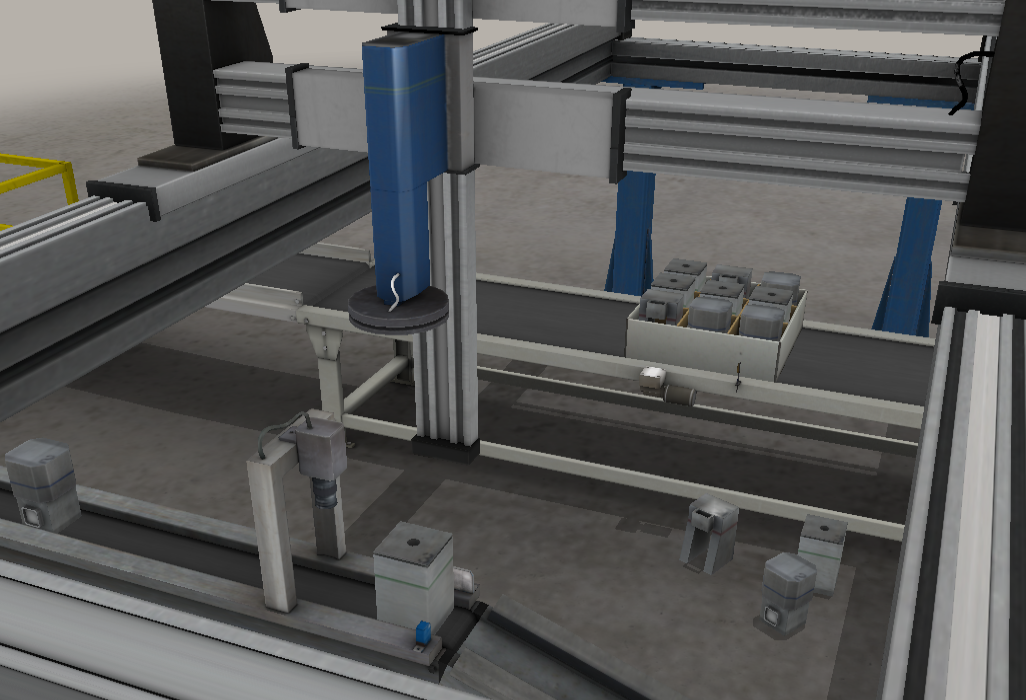
\includegraphics[width=13cm]{titlepage.PNG}\\
			\vspace{\fill}
			\textbf{Novembre 2021}\\
		\end{center}
	\end{titlepage}
	
	\tableofcontents
	\newpage
	
	\section{Introduction}
	
	\section{Composants de base}
		\subsection{Préhensement}
		
		\subsection{Placement de pièce}
	
	\section{Une pièce par boîte}
		\subsection{Admission de pièces}
		
		\subsection{Déplacement vers la boîte}
	
	\section{Remplissage d'une boîte}
		\subsection{Nouveau programme de déplacement}

	\section{Tri par type de pièce}
		\subsection{Nouvelle admission de pièces}
		
		\subsection{Ajustement du programme de déplacement}
	
	\section{Conclusion}
	
\end{document}
